
\documentclass{article}
\usepackage{amsmath}
\usepackage{amsfonts}
\usepackage{amssymb}
\usepackage{graphicx}
\usepackage{tikz}
\usepackage{pgfplots}
\pgfplotsset{compat=1.18}
\begin{document}


\section{TikZ Examples with Tagged Templates}

This document demonstrates TikZ components using the new tagged templates implementation.


\textbf{Geometric Shapes:} Circles, rectangles, lines, and arrows.


\begin{figure}[h]
\centering
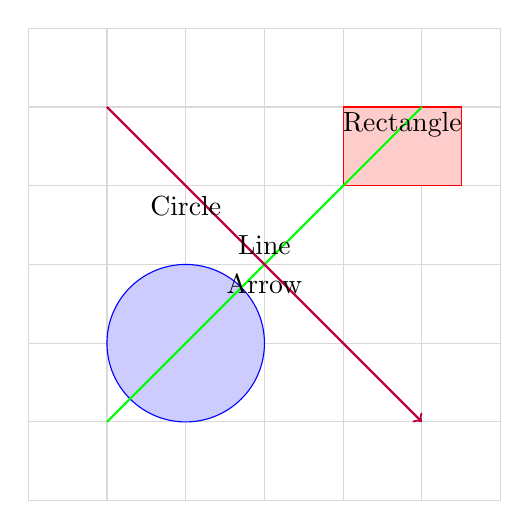
\begin{tikzpicture}[scale=1]
\draw[gray!30][step=1cm] (0,0) grid (6,6);
\draw[fill=blue!20, draw=blue] (2,2) circle (1cm);
\draw[fill=red!20, draw=red] (4,4) rectangle (5.5,5);
\draw[thick, green] (1,1) -- (5,5);
\draw[->, thick, purple] (1,5) -- (5,1);
\node[above] at (2,3.5) {Circle};
\node[above] at (4.75,4.5) {Rectangle};
\node[above] at (3,3) {Line};
\node[below] at (3,3) {Arrow};

\end{tikzpicture}
\end{figure}


\textbf{Mathematical Diagram:} Axes and coordinate system.


\begin{figure}[h]
\centering
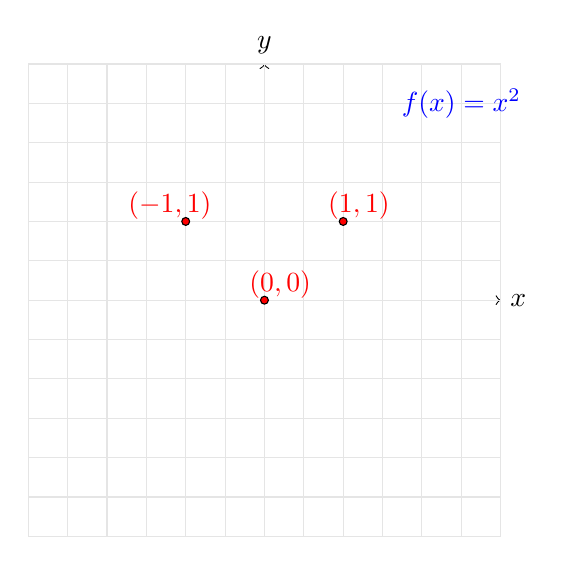
\begin{tikzpicture}[scale=1]
\draw [->] (-3,0) -- (3,0) node[right] {$x$};
\draw [->] (0,-3) -- (0,3) node[above] {$y$};
\draw[gray!20][step=0.5cm] (-3,-3) grid (3,3);
\draw[fill=red] (0,0) circle (0.05cm);
\draw[fill=red] (1,1) circle (0.05cm);
\draw[fill=red] (-1,1) circle (0.05cm);
\node[blue] at (2.5,2.5) {$f(x) = x^2$};
\node[red] at (0.2,0.2) {$(0,0)$};
\node[red] at (1.2,1.2) {$(1,1)$};
\node[red] at (-1.2,1.2) {$(-1,1)$};

\end{tikzpicture}
\end{figure}



\end{document}